\section{Referencia de la Estructura token}
\label{structtoken}\index{token@{token}}
Clase de almacenamiento de raiz de una lista enlazada de Tokens a imprimir con el comando Print en el AST.  


{\tt \#include $<$ast.h$>$}

Diagrama de colaboraci\'{o}n para token:\begin{figure}[H]
\begin{center}
\leavevmode
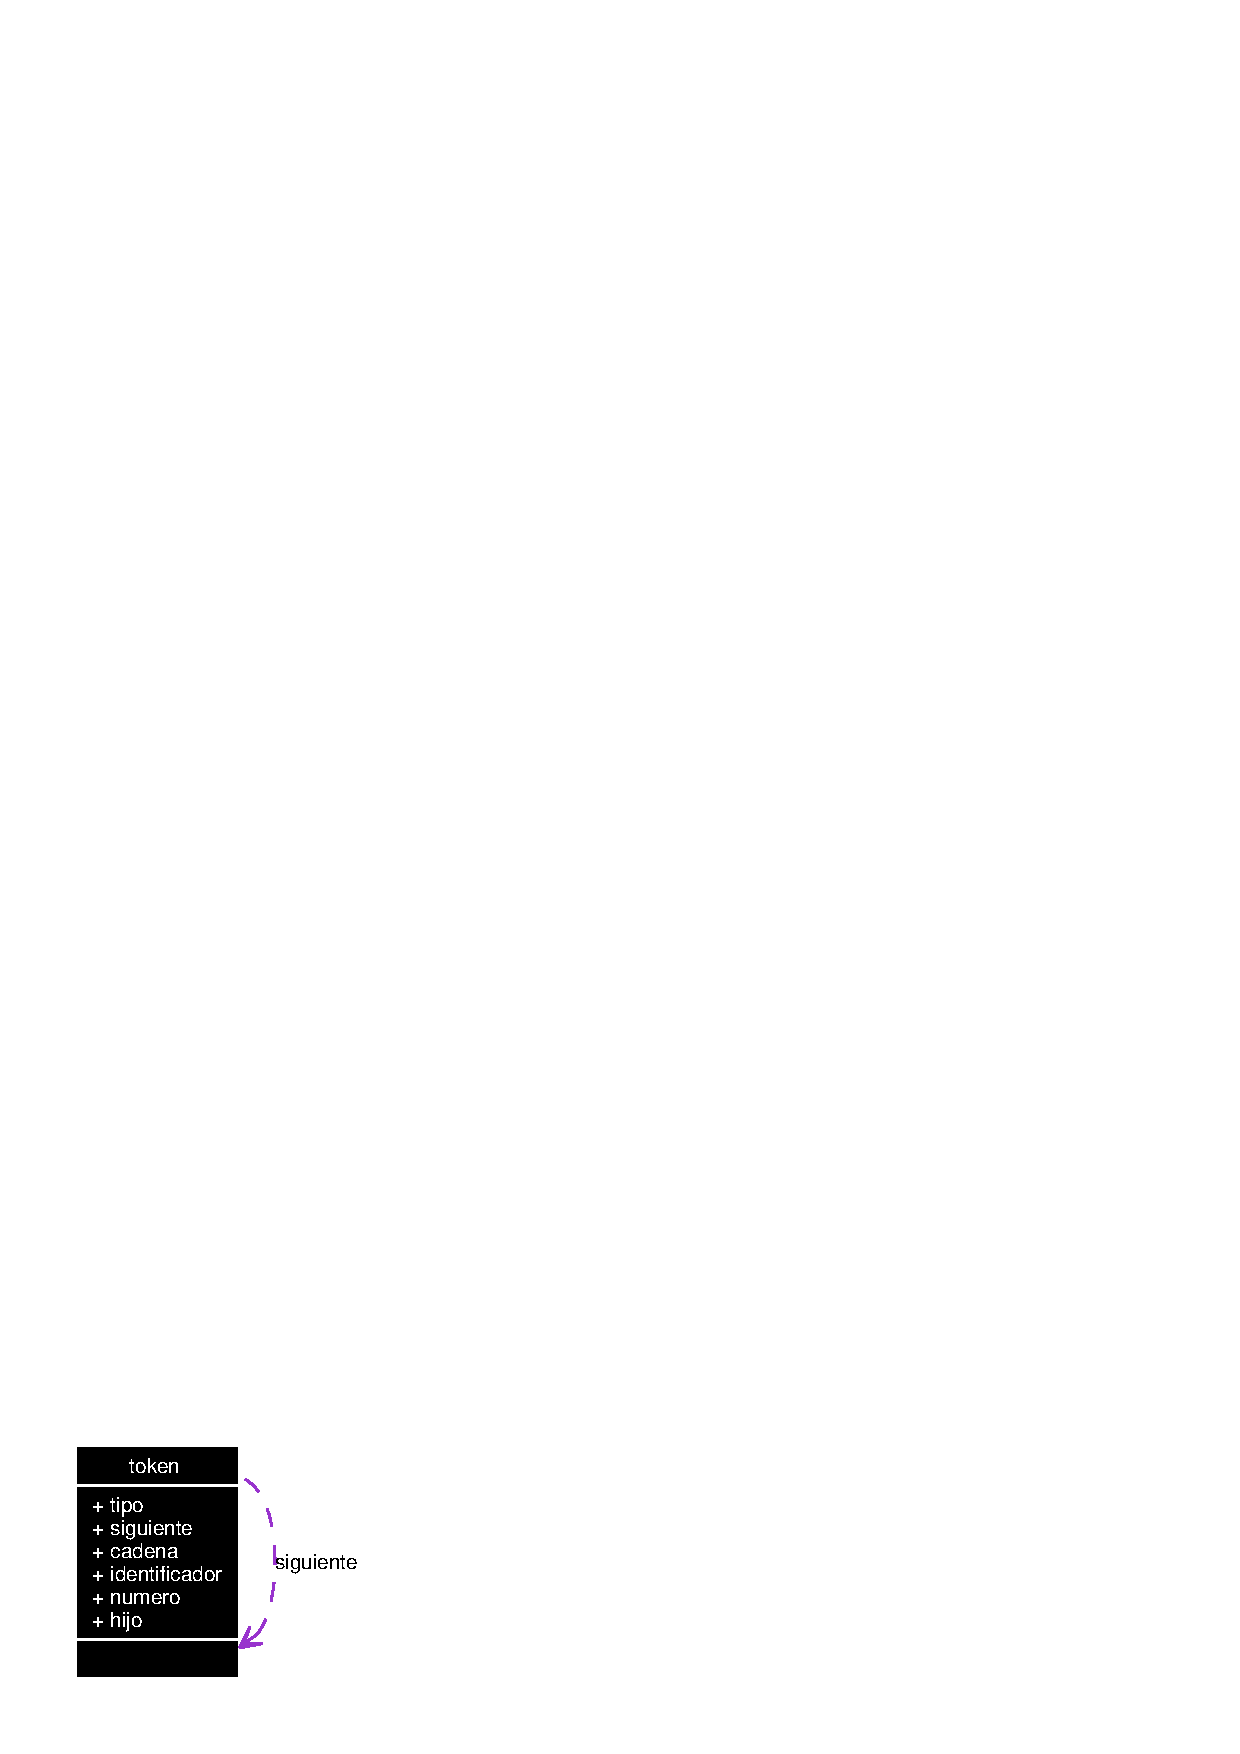
\includegraphics[width=86pt]{structtoken__coll__graph}
\end{center}
\end{figure}
\subsection*{Atributos p\'{u}blicos}
\begin{CompactItemize}
\item 
int {\bf tipo}
\begin{CompactList}\small\item\em Tipo de token a evaluar. \item\end{CompactList}\item 
{\bf token} $\ast$ {\bf siguiente}
\begin{CompactList}\small\item\em puntero a token siguiente en la lista \item\end{CompactList}\item 
\begin{tabbing}
xx\=xx\=xx\=xx\=xx\=xx\=xx\=xx\=xx\=\kill
union \{\\
\>char $\ast$ {\bf cadena}\\
\>char $\ast$ {\bf identificador}\\
\>int {\bf numero}\\
\} {\bf hijo}\\

\end{tabbing}\begin{CompactList}\small\item\em puntero a token \item\end{CompactList}\end{CompactItemize}


\subsection{Descripci\'{o}n detallada}
Clase de almacenamiento de raiz de una lista enlazada de Tokens a imprimir con el comando Print en el AST. 



Definici\'{o}n en la l\'{\i}nea 243 del archivo ast.h.

\subsection{Documentaci\'{o}n de los datos miembro}
\index{token@{token}!cadena@{cadena}}
\index{cadena@{cadena}!token@{token}}
\subsubsection{\setlength{\rightskip}{0pt plus 5cm}char$\ast$ {\bf token::cadena}}\label{structtoken_o2}




Definici\'{o}n en la l\'{\i}nea 247 del archivo ast.h.\index{token@{token}!hijo@{hijo}}
\index{hijo@{hijo}!token@{token}}
\subsubsection{\setlength{\rightskip}{0pt plus 5cm}union \{ ... \}  {\bf token::hijo}}\label{structtoken_o5}


puntero a token 



Referenciado por borrar\-Tokens(), imprimir\-Tokens(), y insertar\-Token().\index{token@{token}!identificador@{identificador}}
\index{identificador@{identificador}!token@{token}}
\subsubsection{\setlength{\rightskip}{0pt plus 5cm}char$\ast$ {\bf token::identificador}}\label{structtoken_o3}




Definici\'{o}n en la l\'{\i}nea 248 del archivo ast.h.\index{token@{token}!numero@{numero}}
\index{numero@{numero}!token@{token}}
\subsubsection{\setlength{\rightskip}{0pt plus 5cm}int {\bf token::numero}}\label{structtoken_o4}




Definici\'{o}n en la l\'{\i}nea 249 del archivo ast.h.\index{token@{token}!siguiente@{siguiente}}
\index{siguiente@{siguiente}!token@{token}}
\subsubsection{\setlength{\rightskip}{0pt plus 5cm}{\bf token}$\ast$ {\bf token::siguiente}}\label{structtoken_o1}


puntero a token siguiente en la lista 



Definici\'{o}n en la l\'{\i}nea 245 del archivo ast.h.

Referenciado por borrar\-Tokens(), concatenar\-Tokens(), imprimir\-Tokens(), y insertar\-Token().\index{token@{token}!tipo@{tipo}}
\index{tipo@{tipo}!token@{token}}
\subsubsection{\setlength{\rightskip}{0pt plus 5cm}int {\bf token::tipo}}\label{structtoken_o0}


Tipo de token a evaluar. 



Definici\'{o}n en la l\'{\i}nea 244 del archivo ast.h.

Referenciado por borrar\-Tokens(), imprimir\-Tokens(), y insertar\-Token().

La documentaci\'{o}n para esta estructura fu\'{e} generada a partir del siguiente archivo:\begin{CompactItemize}
\item 
/media/docs/progra/c++/compiladores1/proy2/godzilla/src/{\bf ast.h}\end{CompactItemize}
